% #############################################################################
% This is Chapter 6
% !TEX root = ../main.tex
% #############################################################################
% Change the Name of the Chapter i the following line
\fancychapter{System Evaluation}
\cleardoublepage
% The following line allows to ref this chapter
\label{chap:evaluation}

This chapter outlines the system evaluation. It is evaluated regarding performance and fullfilled requirements from the previous report and chapter ~\ref{chap:problem}.
The performance tests discusses the objective, tests configuration, results and conclusions.
% -----------------------------------------------------
% -----------------------------------------------------
\section{Communications Performance}\label{chap:evaluation:comms}

Firstly, the performance of the communication channel was tested. Beyond testing the channel performance, it allows to test the performance of the individual services without the communication component. 
The client interface and HSM device communicate through a \ac{UART} serial port.
The performance metrics measured are the average time of data transmission and channel throughput.

% -----------------------------------------------------
\subsection{Testing configuration}\label{chap:evaluation:comms:config}

Only two program are running on the computer while performing the tests, the client program and the SoftConsole IDE needed to run the code on the smartfusion board.
The serial port UART connection is configured with 115200 bit baud rate, 8 data bits, no parity bits and one stop bit.
The elapsed time is measured through two calls to the function \texttt{gettimeofday()} in the C library \texttt{sys/time.h}.

The test was setup on the client application. The application sends a message to the device. It is sent back by the device after reception. The two calls to the time functions are performed in the client application right before sending and after receiving the original message.

The message size was varied to study the performance and scalability of the serial port. For each message size, the test is repeated thirty times and the average time is taken from all repetitions.

% -----------------------------------------------------
\subsection{Results}\label{chap:evaluation:comms:results}

\begin{figure}[h!]
	\centering
	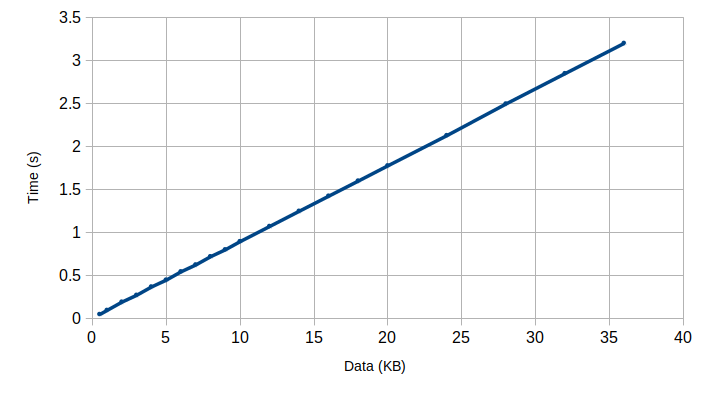
\includegraphics[width=0.8\textwidth]{./Images/comms-time.png}
	\caption{Serial Port Communications Results}
	\label{fig:performance:comms}
\end{figure}

As seen in figure~\ref{fig:performance:comms}, the average transmittion time ranges from 0.016 seconds for 50 bytes, to 2.6 seconds for 29.3 KBytes.
From the graph we can conclude the performance has linear scalability which is ideal for a system.

\begin{figure}[h!]
	\centering
	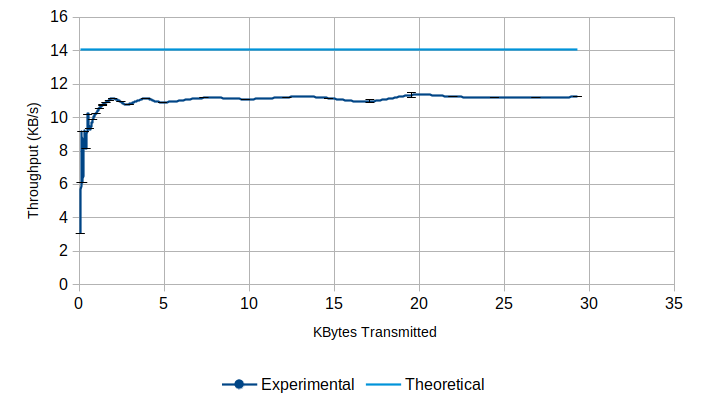
\includegraphics[width=0.8\textwidth]{./Images/comms-tput.png}
	\caption{Serial Port Communications Throughput}
	\label{fig:performance:tput}
\end{figure}

Figure~\ref{fig:performance:tput} plots the experimental throughput and theoretical throughput. The theoretical throughput was calculated from the baud rate \(115200/8 = 14.06 KBytes/s\).
The experimental throughput is 3.05 KB/s for data below 100 bytes and starts stabilizing around 12 KB/s to 11 KB/s as data size increases.
From this we conclude the practical throughput is close to the theoretical, and as expected stabilizes as the sample size increases, meaning, more bytes are transmitted.

% -----------------------------------------------------
% -----------------------------------------------------
\section{Security Services Performance}\label{chap:evaluation:cores}

\subsection{AES-128 and AES-256}\label{chap:evaluation:cores:aes}

% \begin{figure}[h!]
%         \centering     %%% not \center
%         \subfigure[AES 128]{\label{fig:performance:aes128-compare}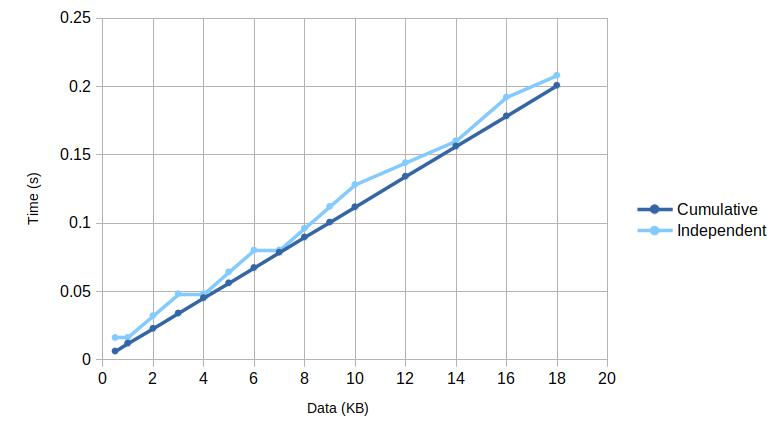
\includegraphics[width=70mm]{Images/aes128-compare.png}}
%         \subfigure[AES 256]{\label{fig:performance:aes256-compare}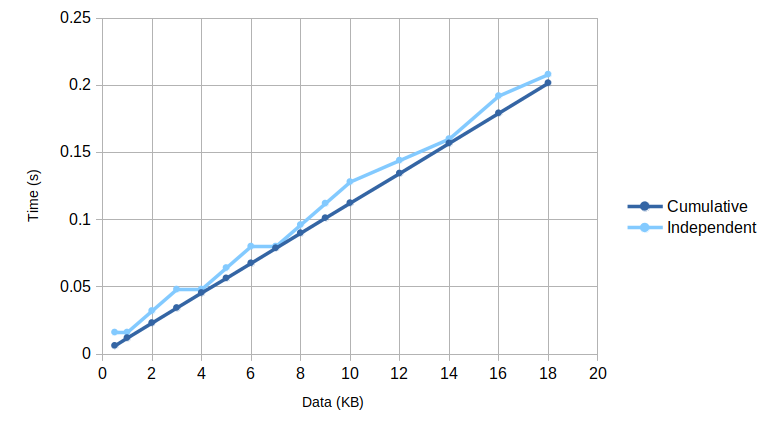
\includegraphics[width=70mm]{Images/aes256-compare.png}}
%         \caption{AES 128 and 256 bit time comparison}
% \end{figure}
\begin{figure}[h!]
	\centering
	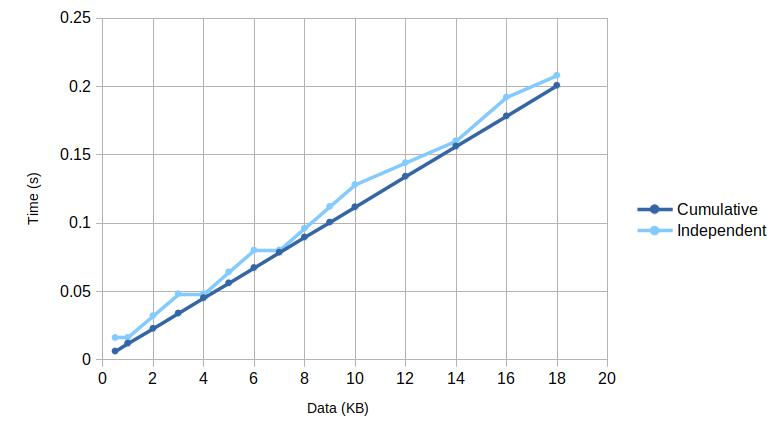
\includegraphics[width=0.9\textwidth]{./Images/aes128-compare.png}
	\caption{AES 128 processing time}
	\label{fig:performance:aes128-compare}
\end{figure}

\begin{figure}[h!]
	\centering
	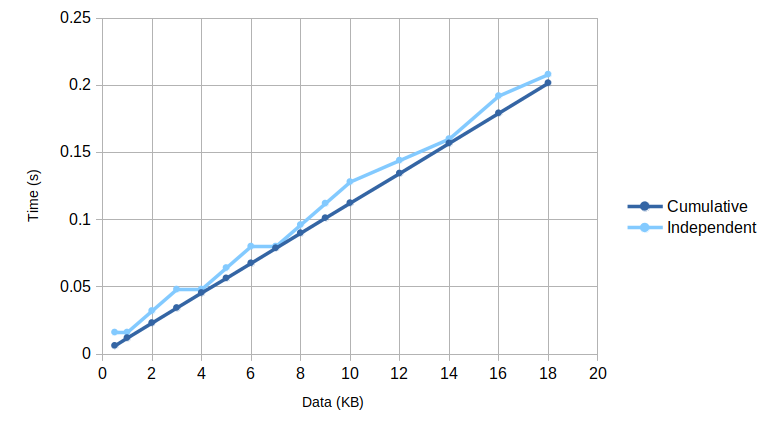
\includegraphics[width=0.9\textwidth]{./Images/aes256-compare.png}
	\caption{AES 256 processing time}
	\label{fig:performance:aes128-compare}
\end{figure}

\begin{figure}[h!]
	\centering
	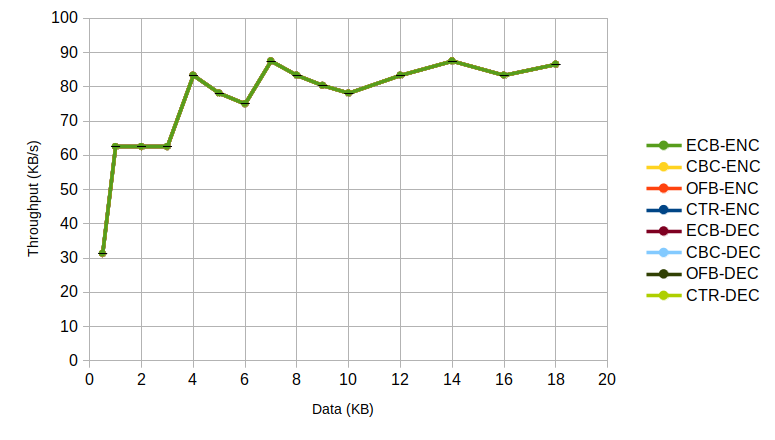
\includegraphics[width=0.9\textwidth]{./Images/aes128-tput.png}
	\caption{AES Throughput}
	\label{fig:performance:aes-tput}
\end{figure}

% -----------------------------------------------------
\subsection{SHA-256 Based Services}\label{chap:evaluation:cores:sha}

\begin{figure}[h!]
	\centering
	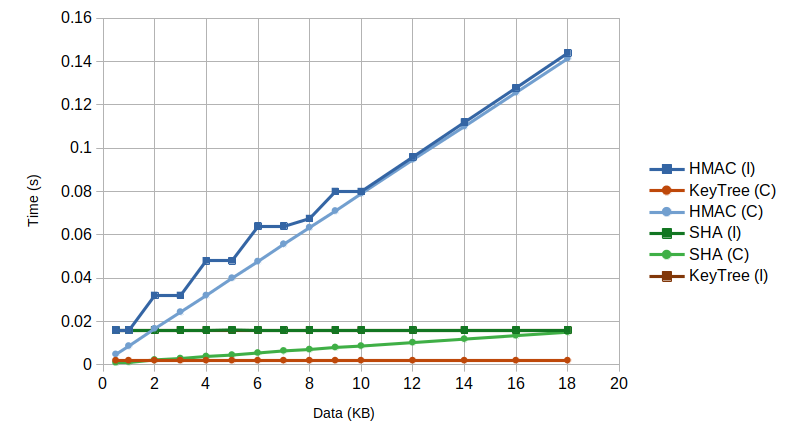
\includegraphics[width=0.9\textwidth]{./Images/sha-compare.png}
	\caption{SHA based services processing time}
	\label{fig:performance:sha-compare}
\end{figure}

\begin{figure}[h!]
	\centering
	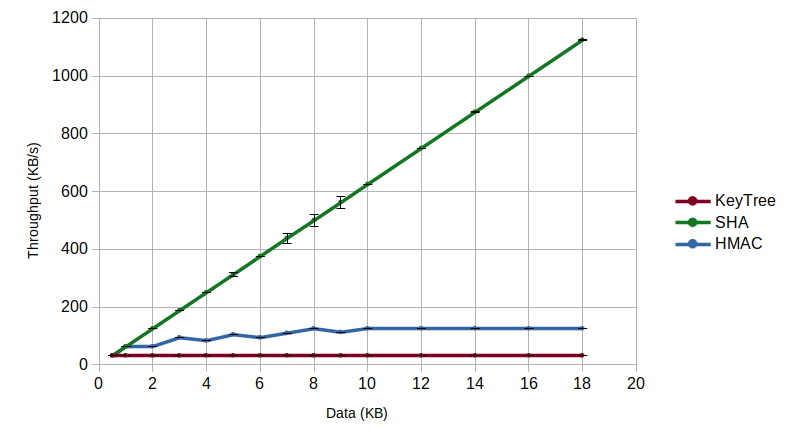
\includegraphics[width=0.9\textwidth]{./Images/sha-tput.png}
	\caption{SHA based services throughput}
	\label{fig:performance:sha-tput}
\end{figure}

% -----------------------------------------------------
% -----------------------------------------------------
\section{Implemented Services Performance}\label{chap:evaluation:services}

The objective of these tests was to measure the performance of the services implemented in the board.
The performance metric measured was the average time to finish the service, excluding the time spent on communications.
The tested services are: data authenticated encryption, data authenticated decryption and new key generation with \ac{ECDH}.

% -----------------------------------------------------
\subsection{Testing Configuration}\label{chap:evaluation:services:config}

The same library used to measure the time in the communication tests was used.
The time was measured at the client application before sending the message which will trigger the service at the HSM, and after it has received the result.

In order to get a real time measurement, each operation was performed 1000 times on the HSM, with the communications only done once.
From the resulting time, the predicted time spent on communications was subtracted using the data from the previous test. The result was then divided by 1000.

The data encryption and decryption operations were ran with different data sizes, in order to asses the data size impact on performance.
The ECDH key generation always uses a private and public key of the same size, so no message size variation is possible.

% -----------------------------------------------------
\subsection{Results}\label{chap:evaluation:services:results}

\begin{table}[h!]
	% \large
	\centering
	\def\arraystretch{1.5}
	\begin{tabular}{|c|c|c|c|c|} \cline{2-5}
		\multicolumn{1}{c|}{} & \multicolumn{2}{c|}{Average Time (s)}  & \multicolumn{2}{c|}{Throughput (KB/s)}\\ \hline
		\centering Data Size (bytes) & Encryption & Decryption & Encryption & Decryption \\ \hline
		79 & \textbf{0.12848} & \textbf{0.12848} & \textbf{0.6} & \textbf{0.6}	      \\ \hline
		500 & \textbf{0.12848} & \textbf{0.12849} & \textbf{3.8} & \textbf{3.8}	      \\ \hline
		1500 & \textbf{0.12853} & \textbf{0.12854} & \textbf{11.4} & \textbf{11.4}	      \\ \hline
		2000 & \textbf{0.12852} & \textbf{0.12851} & \textbf{15.2} & \textbf{15.2}            \\ \hline
	\end{tabular}
	\caption{Encryption/Decryption Performance.}
	\label{tab:data-performance}
\end{table}


The results in table~\ref{tab:data-performance} for the encryption and decryption operations are very similar due to both using the same board services, AES encryption and HMAC, but in a different order. It is also important to note AES encryption and decryption in CTR mode is essentially the same operation due the mode's characteristics.
Relating to the variation in data size, the values vary between approximately 0.1284 and 0.1825 seconds, which is a very insignificant difference. Thus we can conclude, the data size has a negligible impact on the operations performance.

\begin{table}[h!]
	\centering
	\def\arraystretch{1.5}
	\begin{tabular}{|l|l|} \cline{2-2}
	\multicolumn{1}{l|}{} & Average Time (s)  \\ \hline
		\begin{tabular}[c]{@{}l@{}}1000 reps w/o\\ enroll key\end{tabular} & \textbf{0.577155101462}     \\ \hline
			\begin{tabular}[c]{@{}l@{}}10 resp w/ \\enroll key\end{tabular}    & \textbf{1.7636150462}       \\ \hline
	\end{tabular}
	\caption{ECDH Performance.}
	\label{tab:ecdh-performance}
\end{table}


Regarding the key generation operation results in table~\ref{tab:data-performance}, two values were obtained through different methods. Due to the operation using SRAM-PUF services to enroll new keys in the eNVM memory, with limited write cycles and key slots, this operation cannot be repeated enough times to get a relevant enough sample size.
So a trade off was achieved. The operation was performed 1000 times without the key enrollment operation, meaning only the ecdh key generation algorithm and key derivation function (SHA-256).
Since the enrollment phase is presumed to be expensive, due to writing in eNVM memory, the test was also performed 10 times with key enrollment, to get an idea of its potential performance cost.

A higher time of 0.577 seconds without enrollment and 1.764s with, compared to the previous operations is expected due to the higher cost of operations with asymmetric keys.
However, comparing both values we can conclude saving the key in memory, has most likely the higher performance impact on the operation.
This result is congruent with the one obtained by \cite{parrinha2017flexible} of 0.57s per ECC scalar multiplication.
Thus we can conclude, the scalar multiplication is the second most expensive operation, after the key enrollment, since the key derivation function has a negligible impact on the processing time (0.577s with the function vs 0.57s without).

% -----------------------------------------------------
% -----------------------------------------------------
\section{Requirements}\label{chap:evaluation:requirements}

A M2S090TS smartfusion2 evaluation kit is priced at 384€ \cite{smartfusionPrice}.

% ------------- Requirements ------------------
% Devices should be distributable to individuals or entities with one or more individuals;
% The system must allow communications between individuals representing themselves or an entity;
% The system must be responsible for securing all communications against any sort of attacks;
% The device should be independent from user's personal computers;
% Users should be able to create secure communications with available and new entities;
% m New secure connections should be created, if existing communications are suspected to be compromised;
% It should provide an easy-to-use interface by everyone, including non-technical people;
% It should have a relatively low cost, to allow distribution of several devices among multiple people;
% Only authorized individuals should be able to use the device.
% ---------------------------------------------

% secure comms - aes and hmac services are not dpa resistant, so keys should be regularly replaced to avoid enough data which enables an attacker to break encryption. On the other hand this is only possible if the attacker has physical access to the device or potentially with some type of malware on the user's computer.
% key generation - needs assymetric keys to generate new keys with public keys and salt traded beforehand - can be not user friendly
